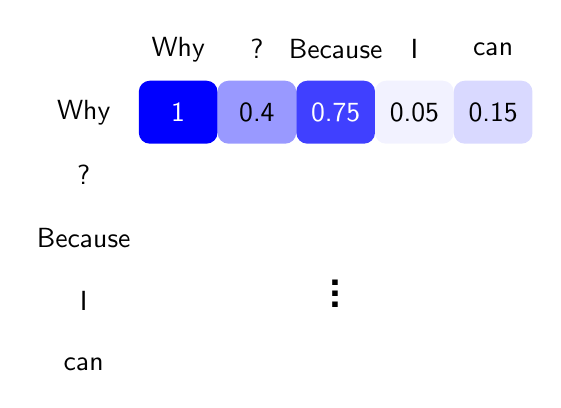
\begin{tikzpicture}[
    y=-1cm,
    every node/.style={font=\sffamily},
    matrixc/.style={fill=blue,rounded corners,minimum height=0.8cm, minimum width=1cm},
]

    \node (why) at (0, 0.8) {Why};
    \node (int) at (0, 1.6) {?};
    \node (because) at (0, 2.4) {Because};
    \node (i) at (0, 3.2) {I};
    \node (can) at (0, 4.0) {can};

    \node (why2) at (1.2, 0) {Why};
    \node (int2) at (2.2, 0) {?};
    \node (because2) at (3.2, 0) {Because};
    \node (i2) at (4.2, 0) {I};
    \node (can2) at (5.2, 0) {can};

    \node[matrixc, text=white] (ww) at (1.2, 0.8) {1};
    \node[matrixc, fill=blue!40] (wint) at (2.2, 0.8) {0.4};
    \node[matrixc, fill=blue!75, text=white] (wb) at (3.2, 0.8) {0.75};
    \node[matrixc, fill=blue!5] (wi) at (4.2, 0.8) {0.05};
    \node[matrixc, fill=blue!15] (wc) at (5.2, 0.8) {0.15};

    % node big dots (...) in matrix middle
    \node (dots) at (3.2, 3) {\Huge $\vdots$};

\end{tikzpicture}
